\section{Obiettivi}
Questa esercitazione mira ad implementare un traduttore automatico
dall'italiano all'inglese basato su \textit{Trasfer Sintattico}\footnote{Approccio simbolico ben noto in letteratura definito da Vaquois nel suo triangolo\cite{book}}.
\begin{figure}[ht]
	\centering 
	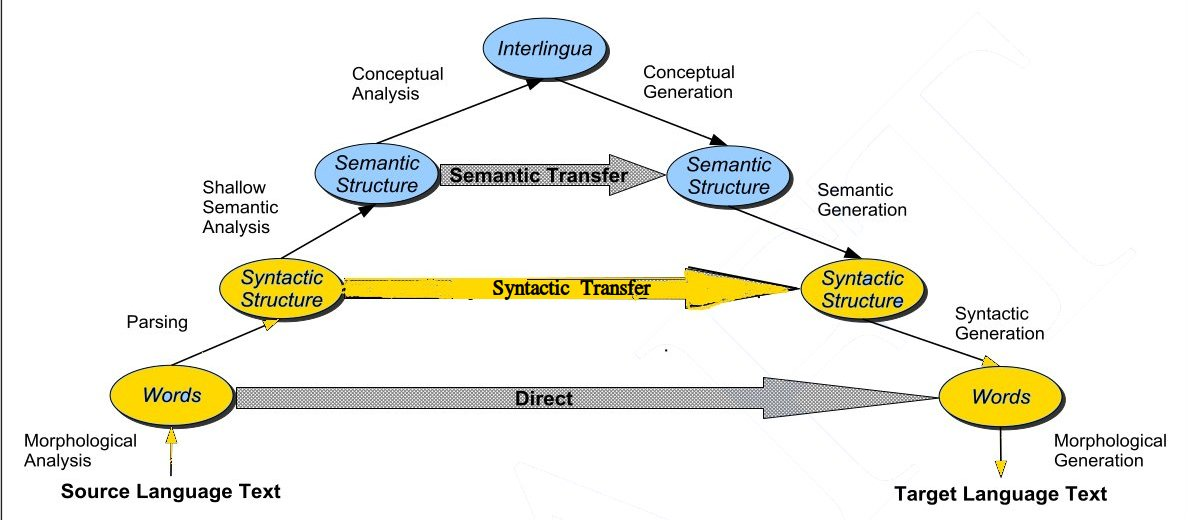
\includegraphics[scale=0.25]{./img/TransferSintattico}
	\caption{Il triangolo di Vauquois (1968)}
	\label{Vauquois_triangle}
\end{figure}\\
Come evidenziato in Figura \ref{Vauquois_triangle}, il processo sotteso al suddetto paradigma consta 
nell'analizzare morfologicamente la frase in input, costruire il relativo albero di parsing, applicare ad esso opportune regole di trasformazione volte alla costruzione di una struttura sintattica per la lingua target, ponendo quindi le basi per la generazione della frase tradotta. \\
Ciascuna fase del processo verrà analizzata nel dettaglio nelle successive sezioni, prestando particolare attenzione alle strutture dati impiegate ed ai dettagli implementativi rilevanti. L'intera pipeline di elaborazione è stata implementata
nel linguaggio Java. 

\subsection{Requisiti}
\label{sec:requisiti}
La Traduzione automatica è un task intrinsecamente difficile, ancora oggi i moderni traduttori non sono in grado si svolgere pienamente quella \textit{letteraria} \cite{book}. \\
L'esercitazione  si pone l'obiettivo di costruire un applicativo in grado di elaborare un numero ben ristretto di frasi della lingua italiana, a tal proposito vengono riportate le specifiche dei vincoli che devono essere soddisfatti dall'input:
\begin{itemize}[label=$\ast$]
	\item Il periodo in ingresso deve essere mono-proposizionale\footnote{Il periodo deve essere composto da una sola proposizione, non sono pertanto ammesse proposizioni subordinate} 
	\item La frase deve essere affermativa
	\item Il verbo deve essere coniugato al modo Indicativo
	\item L'avverbio deve essere un modificatore del verbo
	\item La frase non deve contenere congiunzioni
%	\item L'aggettivo non può essere un modificatore dell'avverbio
	\item I \textbf{lemmi} dei termini della frase devono appartenere al seguente lessico:
	\lstinputlisting[label={lexicon},style = javacode, caption ={Lessico accettato per l'Italiano}]{java/lexicon}  
	
	
\end{itemize}
La violazione di uno o più dei suddetti vincoli comporterà il lancio di un'eccezione custom da parte dell'applicativo. \\
Il programma deve essere dunque in grado di elaborare le seguenti frasi:
\begin{enumerate}[label=(\roman*)]
	\item È la spada-laser di tuo padre
	\item Ho fatto una mossa leale
	\item Gli ultimi avanzi della vecchia Repubblica sono stati spazzati via
\end{enumerate}


